\vspace{-3mm}

\section{Das Vorkurs-Team}
\vspace{-1mm}

\begin{figure*}[!b]
    \centering
    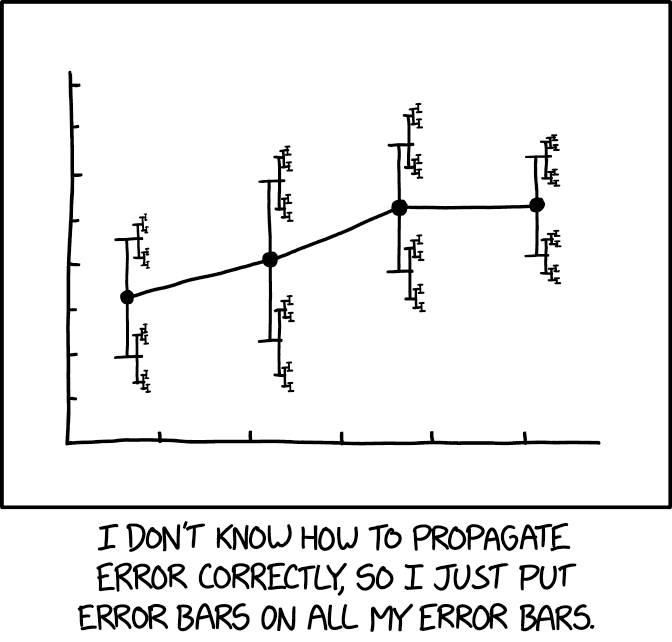
\includegraphics[width=0.5\textwidth]{bilder/error_bars_2x.png}
\end{figure*}

Die Vorkurse für Erstsemester werden von einer kleinen Gruppe an Leuten, die in der Fachschaft MathPhysInfo tätig sind, ehrenamtlich organisiert. Diese kümmern sich um die Planung und Koordination der Fachvorträge und des Rahmenprogramms, damit es zu einem möglichst reibungslosen Ablauf kommt.

Die Fachvorträge der Vorkurse Mathematik und Informatik\footnote{die Vorträge im Physikvorkurs werden seit geraumer Zeit von der Fakultät verantwortet} werden vollständig von Studentinnen der Fachschaft und des „Sympi-Sumpf“\footnote{Gruppe von Alt-Fachschaftlerinnen, Freunden und allen, die der FS nahestehen} ausgearbeitet und gehalten. Darüber hinaus sind viele Studierende der Info, Mathe und Physik als Helfer an der Durchführung der Spieleabende, Kneipentouren und Wanderungen beteiligt. Dieses Engagement erfolgt ehrenamtlich und unabhängig von den beiden Fakultäten. Alles in allem sind mehr als 60 Personen in die Durchführung und Planung des Vorkurs involviert.

Der vor dem Vorkurs stattfindende Programmiervorkurs wird von ein paar Studentinnen verantwortet, die sich auch um das Skript für diesen kümmern.

Wenn du Lust hast, dich im nächsten Jahr beim Vorkurs zu engagieren, komm doch einfach bei einer der Fachschatssitzungen vorbei -- Helferinnen werden immer gebraucht und sind herzlich willkommen. Auch im nächsten Jahr gilt es aufs Neue Spiele zu planen, Referentinnen zu suchen, Räume zu reservieren und sich mit den Fakultäten zu koordinieren.

\vfill\eject
